\title{Chapter 4, Section 1. Exercises 1, 2, 3 and 5}
\author{
	MTH 594, Prof. Mikael Vejdemo-Johansson \\
	Differential Geometry Independent Study \\
	\\
	Matthew Connelly \\
}
\date{\today}



\documentclass[12pt]{article}

\usepackage[top=.5in, bottom=.75in, left=1in, right=1in]{geometry}
\usepackage{amssymb}
\usepackage{amsmath}
\usepackage{graphicx}
\usepackage{subcaption}


\begin{document}
\maketitle

\section*{Exercise 4.1.3}

The \emph{hyperboloid of one sheet} is
$$
S = \lbrace \left( x,y,z \right) \in \mathbb{R}^3 \ \vert \ x^2 + y^2 - z^2 = 1  \rbrace.
$$

Show that, for every $\theta$, the straight line
$$
(x-z)cos\theta = (1-y)sin\theta,  \ (x+z)sin\theta = (1+y)cos\theta
$$

is contained in $S$, and that every point of the hyperboloid lies on one of these lines. Deduce that $S$ can be covered by a single surface patch, and hence is a surface. (Compare the case of the cylinder in Example 4.1.3.)
\\\\
\indent
Find a second family of straight lines on $S$, and show that no two lines of the same family intersect, while every line of the first family intersects every line of the second family with one exception. One says that the surface $S$ is doubly ruled.

\vspace{1cm}
\hrule
\vspace{1cm}

\noindent
\underline{Lines in hyperboloid $S$:}\\\\
\indent
The line mentioned in the problem can be parametrized as
$$
r = (cos\theta - sin\theta \ t, sin\theta + cos\theta \ t, t)
$$
\clearpage
When rotated about a unit circle in the $xy$-plane, $r$ will trace out a hyperboloid of one sheet.
\begin{figure}[h!]
  \centering
      \begin{subfigure}[b]{0.6\linewidth}
    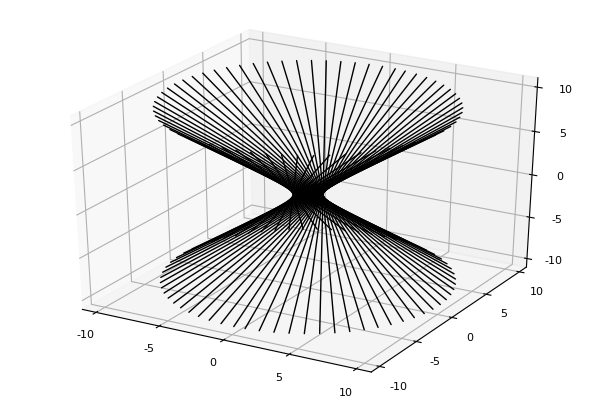
\includegraphics[width=\linewidth]{./assets/4-1-3/hyperboloid-line-rotation.png}
    \caption*{A collection of $r$ lines at various points of rotation.}
  \end{subfigure}
  \end{figure}
  
  \indent
  All points within $S$ will lie on one of these lines after a single period of rotation \newline $\theta \in [0,2\pi)$. Then, for a homeomorphism $\sigma$: by restricting $\sigma$'s domain to a open interval of $(0,2\pi)$ (similar to a single period of $r$'s rotation), $\sigma$ will be made injective. Then, for an open disc $U \in \mathbb{R}^2$,
   $$
  U = \lbrace (x,y) \in \mathbb{R}^2  \ \vert \ x^2 + y^2 > 1\rbrace 
  $$
  $$
  \sigma : U \rightarrow S
  $$

showing $S$ to be coverable by a single surface patch $\sigma$.

\begin{figure}[h!]
  \centering
      \begin{subfigure}[b]{0.6\linewidth}
    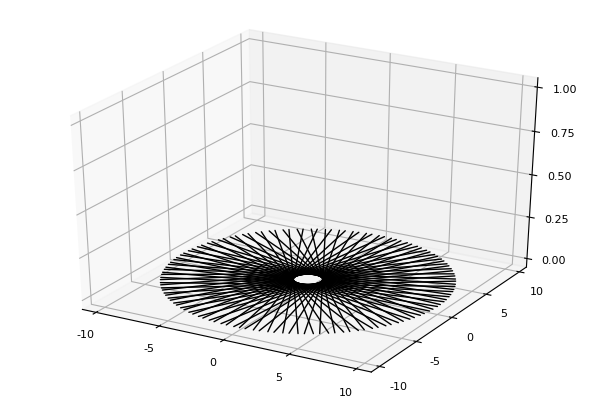
\includegraphics[width=\linewidth]{./assets/4-1-3/hyperboloid-line-rotation-planar.png}
    \caption*{Lines in $U$, rotated about $x^2+y^2=1$, similar to $r$.}
  \end{subfigure}
  \end{figure}


\clearpage
\begin{figure}[h!]
  \centering
      \begin{subfigure}[b]{0.6\linewidth}
    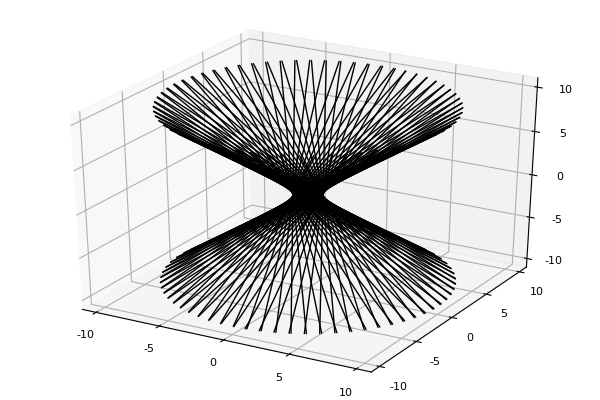
\includegraphics[width=\linewidth]{./assets/4-1-3/hyperboloid-line-rotation-skew.png}
    \caption*{A collection of $r_2$ lines, intersecting $r$.}
  \end{subfigure}
  \end{figure}

\end{document}
This is never printed